\documentclass[compress]{beamer}
\usepackage{lmodern} % Fixing beamer issues
\usepackage[T1]{fontenc}
%%% Support some german text
% \usepackage{ngerman}
% \usepackage[latin1]{inputenc}   % für Umlaute
%%%
\usepackage[utf8]{inputenc}
%%%
\usepackage[english]{babel}
\usepackage{amsmath}
\usepackage{amsfonts}
% \usepackage[inline]{enumitem} % To get roman numbers, breaks normal arrows...
\usepackage{microtype}
% \usepackage{eulervm}
% \usepackage{array} % needed for \arraybackslash
% \usepackage{graphicx}
% \usepackage{adjustbox} % for \adjincludegraphics
% \usepackage{soul}
\usepackage{color}
% \usepackage{animate}

% \usepackage{../../TesiTriennale/Manoscritto/Styles/commands}
\definecolor{mygreen}{rgb}{0,0.6,0}
\definecolor{mygray}{rgb}{0.4,0.4,0.4}
\definecolor{mymauve}{rgb}{0.58,0,0.82}
\usepackage{listings}
\lstset{ 
  % backgroundcolor=\color{white},   % choose the background color; you must add \usepackage{color} or \usepackage{xcolor}; should come as last argument
  basicstyle=\tiny,        % the size of the fonts that are used for the code
  breakatwhitespace=true,         % sets if automatic breaks should only happen at whitespace
  breaklines=true,                 % sets automatic line breaking
  captionpos=b,                    % sets the caption-position to bottom
  commentstyle=\color{mygreen},    % comment style
  % deletekeywords={...},            % if you want to delete keywords from the given language
  escapeinside={\%*}{*)},          % if you want to add LaTeX within your code
  % extendedchars=true,              % lets you use non-ASCII characters; for 8-bits encodings only, does not work with UTF-8
  frame=single,	                   % adds a frame around the code
  keepspaces=true,                 % keeps spaces in text, useful for keeping indentation of code (possibly needs columns=flexible)
  keywordstyle=\color{blue},       % keyword style
  language=C,                 % the language of the code
  % morekeywords={*,...},            % if you want to add more keywords to the set
  numbers=left,                    % where to put the line-numbers; possible values are (none, left, right)
  numbersep=5pt,                   % how far the line-numbers are from the code
  numberstyle=\tiny\color{mygray}, % the style that is used for the line-numbers
  rulecolor=\color{gray},         % if not set, the frame-color may be changed on line-breaks within not-black text (e.g. comments (green here))
  showspaces=false,                % show spaces everywhere adding particular underscores; it overrides 'showstringspaces'
  showstringspaces=false,          % underline spaces within strings only
  showtabs=false,                  % show tabs within strings adding particular underscores
  stepnumber=1,                    % the step between two line-numbers. If it's 1, each line will be numbered
  stringstyle=\color{mymauve},     % string literal style
  tabsize=2,	                   % sets default tabsize to 2 spaces
  % title=\lstname                   % show the filename of files included with \lstinputlisting; also try caption instead of title
}


\newcommand{\nota}[1]{\textcolor{red}{#1}}

\title[]{How runtime systems can support resource awareness in HPC: the HPX case}
\author{Tommaso Bianucci}
\date{22 June 2018}
\institute{Technische Universität München}
%\logo{\includegraphics[width=15mm]{logo}}
\usetheme{Dresden}
% \usecolortheme{beaver}
%\useoutertheme[right]{sidebar}
\setbeamercovered{dynamic}
% \setbeamertemplate{theorems}[numbered]
% \theoremstyle{definition}
% \newtheorem{definizione}{Definizione}
% \theoremstyle{plain}
% \newtheorem{teorema}{Teorema}

% Mastruzzo per poter controllare gli odiosi pallini di navigazione
\makeatletter
\let\beamer@writeslidentry@miniframeson=\beamer@writeslidentry
\def\beamer@writeslidentry@miniframesoff{%
  \expandafter\beamer@ifempty\expandafter{\beamer@framestartpage}{}% does not happen normally
  {%else
    % removed \addtocontents commands
    \clearpage\beamer@notesactions%
  }
}
\newcommand*{\miniframeson}{\let\beamer@writeslidentry=\beamer@writeslidentry@miniframeson}
\newcommand*{\miniframesoff}{\let\beamer@writeslidentry=\beamer@writeslidentry@miniframesoff}
\makeatother
% 
\begin{document}

\begin{frame}
\maketitle
\end{frame}

\section{Introduction}
\begin{frame}
	\frametitle{Exascale will be hard}
	\begin{itemize}
		\item $1$ ExaFLOPS = $10^{18}$ FLOPS
		\item Billions of cores?
		% \item $10^4$ nodes
		\item Etherogeneous hardware
		\begin{itemize}
			\item Manycore CPUs
			\item GPUs
			\item FPGAs
		\end{itemize}
	\end{itemize}
	\pause
	\vspace{5mm}
	$\longrightarrow$ These machines expose an extreme degree of parallelism.
\end{frame}

\begin{frame}
	\frametitle{Applications are hard}
	\begin{itemize}
		\item \emph{Scaling-impaired} applications
		% Esempio?
		\item Unbalanced execution tree
		% Qui esempio e' AMR
	\end{itemize}
	\pause
	This causes:
	\begin{itemize}
		\item Poor parallel performance
		\item Suboptimal resource usage
	\end{itemize}
	\pause
	\vspace{5mm}
	$\longrightarrow$ Some applications do not scale well.
	% e qui spiega cosa vuol dire scalare
\end{frame}

\begin{frame}
	\frametitle{Programming model matters}
	Current predominant model in HPC:
	\begin{itemize}
		\item \emph{Fork-join} for shared memory (OpenMP)
		\pause
		\item \emph{Communicating Sequential Processes} for distributed memory (MPI)
	\end{itemize}
	\pause
	Problems:
	\begin{itemize}
		\item Global barriers
		\item Load imbalance
	\end{itemize}
% We will see an alternative later
\end{frame}

\begin{frame}
	\frametitle{Programming model matters (2)}
	\vspace{-3mm}
	\begin{center}
		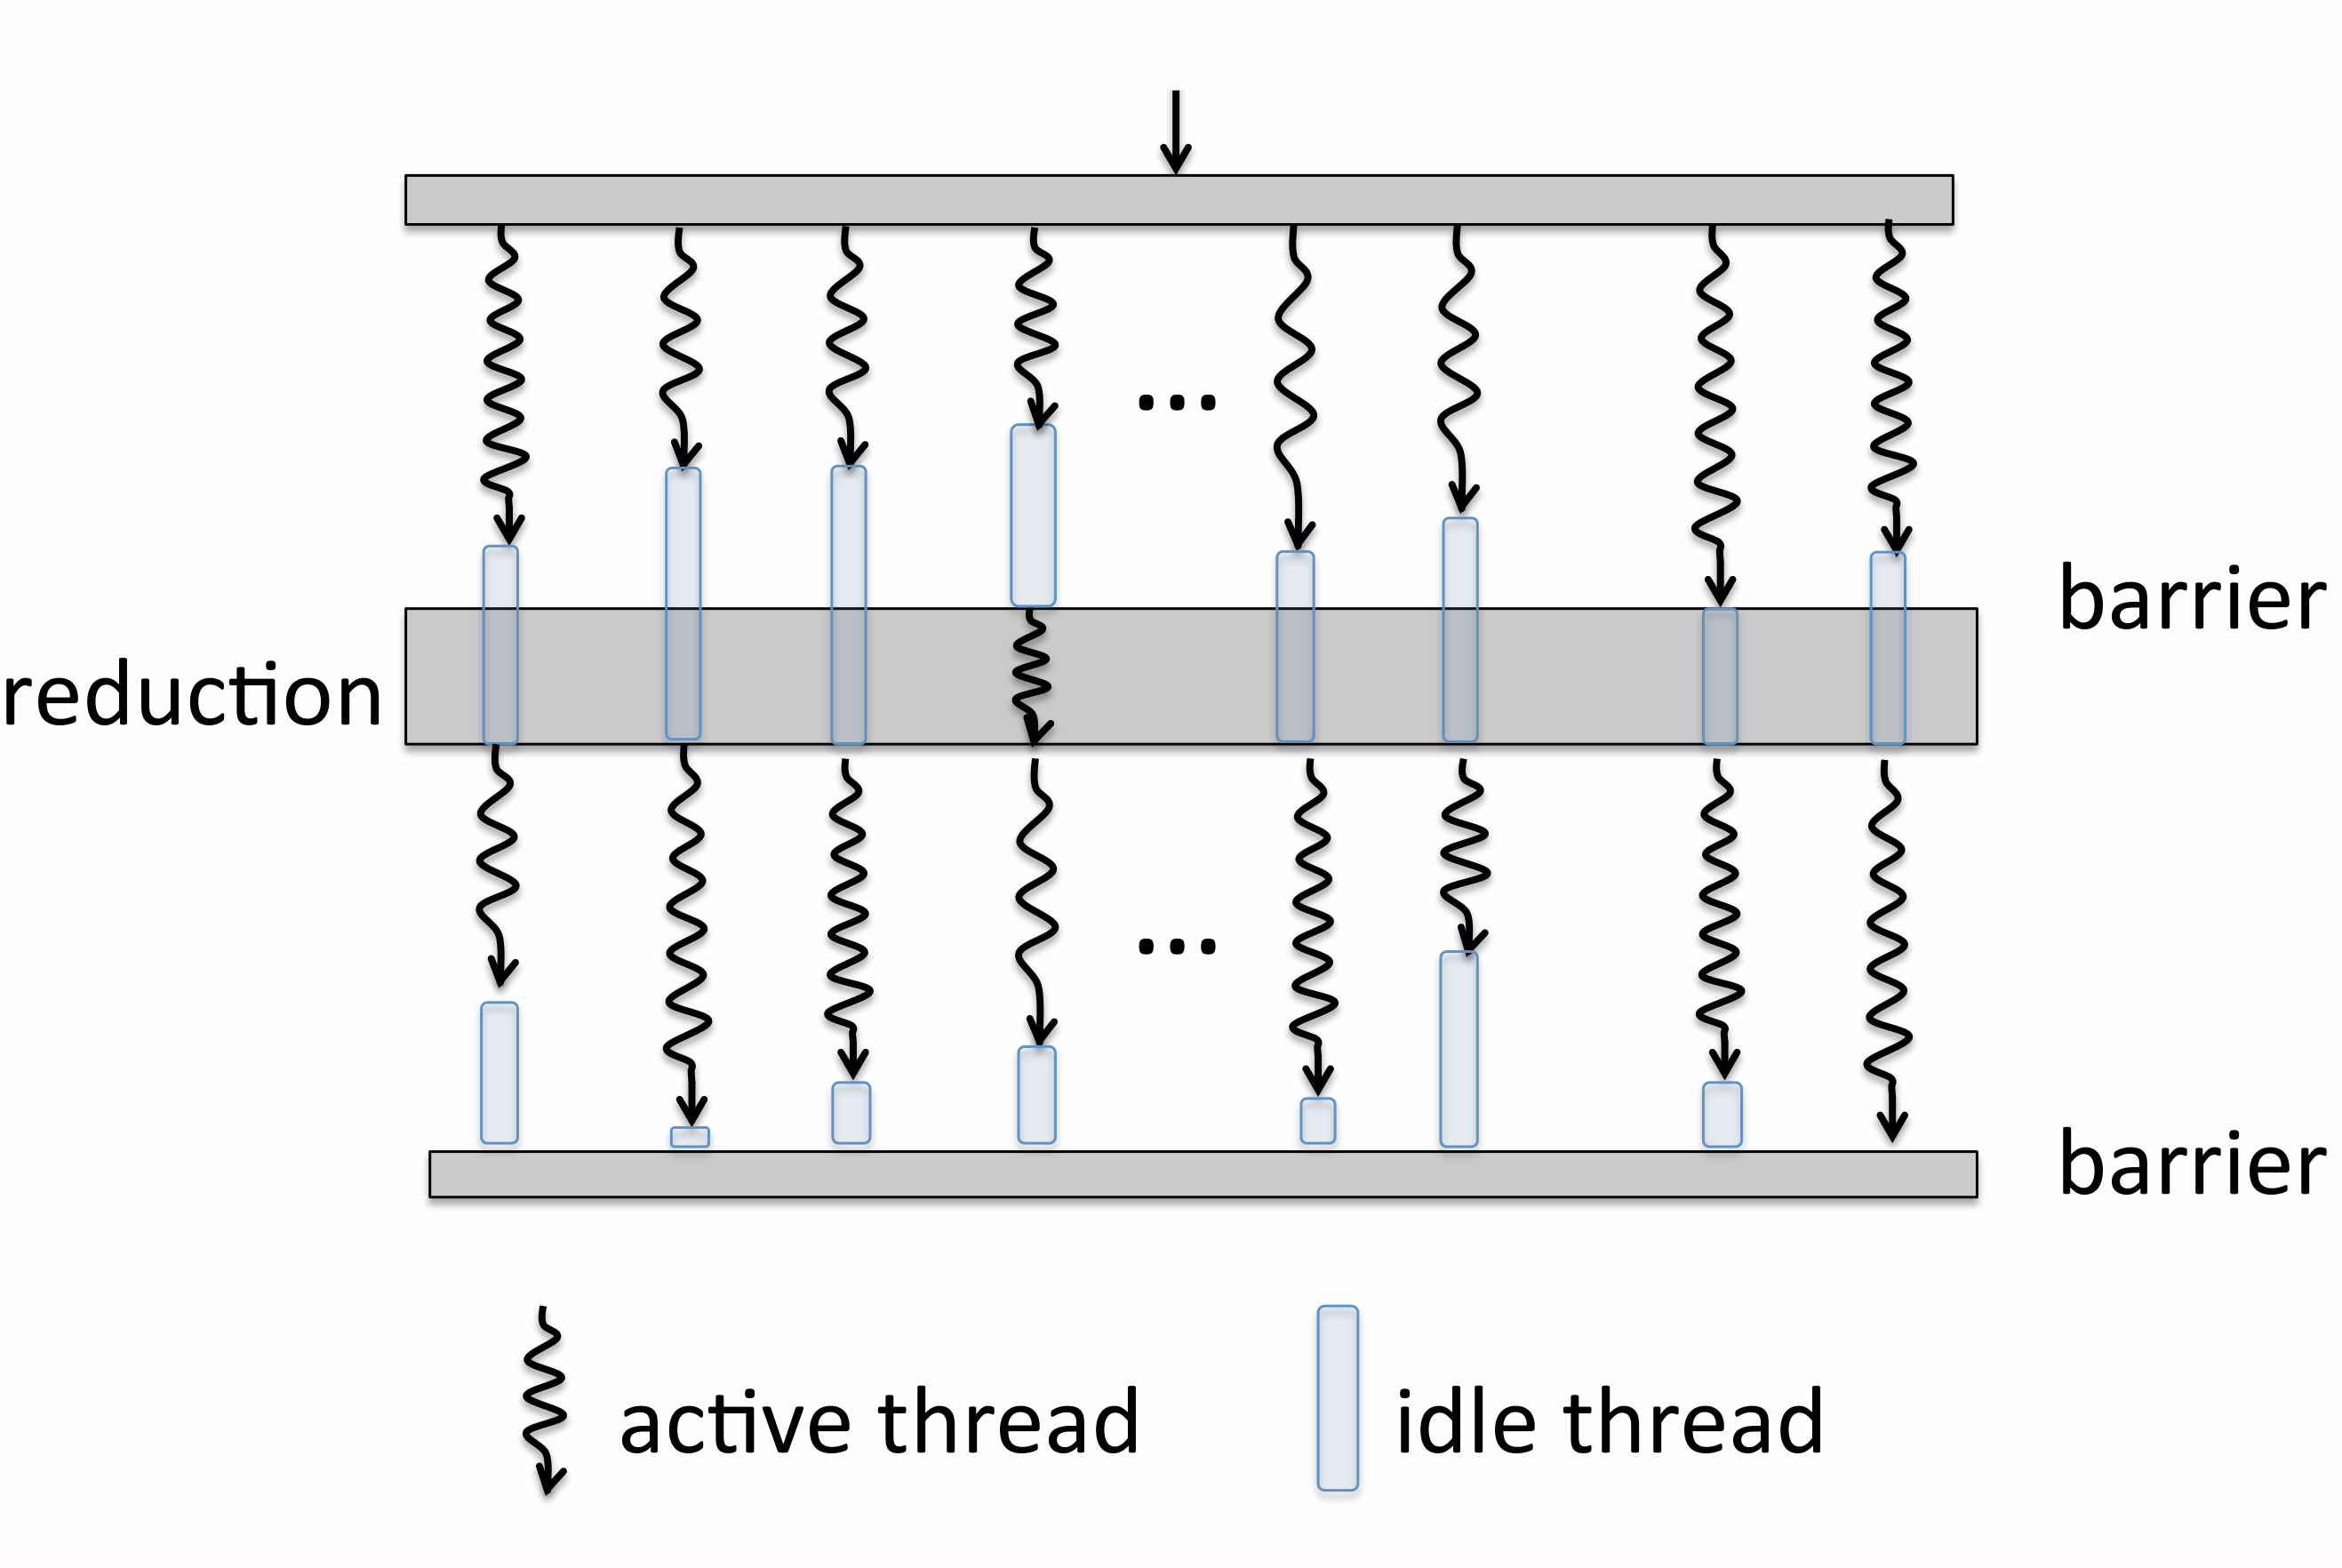
\includegraphics[width=80mm]{Figures/globalBarriersAndThreadIdleTime.png}\\
		\tiny P. A. Grubel: "Dynamic adaptation in hpx - a task-based parallel runtime system" 2016.
		\normalsize
	\end{center}
	\pause
	$\longrightarrow$ Limits of programming models can limit parallelism.
	% e qui spiega cosa vuol dire scalare
	% here it is also important to mention various overheads of parallelization!
\end{frame}

\section{Resource awareness}
\begin{frame}
	% \frametitle{Running blindly does not pay}
	\frametitle{Complex hardware requires clever software}
	\pause
	Resource awareness
	\vspace{5mm}
	\begin{itemize}
		\item Adaptive allocation and usage of resources
		\item The system is aware of its own resources
		\item At runtime vs. before execution
	\end{itemize}
\end{frame}

\begin{frame}
	\frametitle{What are resources?}
	\begin{enumerate}
		\item Hardware entities
			\begin{itemize}
				\item Computational units
				\item Memory
				\item Bus/network bandwidth
				\item I/O devices
				\item Power
				\item Thermal
			\end{itemize}
		\pause
		\item Software entities
			\begin{itemize}
				\item Buffers
				\item Queues
			\end{itemize}
	\end{enumerate}
\end{frame}

\begin{frame}
	\frametitle{Different levels of awareness}
	\begin{enumerate}
		\item Embedded computing
		% Cosa vuol dire di preciso embedded? Che ci scriviamo roba baremetal?
		\begin{itemize}
			\item Deal with power, aging, thermal effects/problems
			\item Manage low-level access to resources\\
			E.g.: Invasive computing on MPSoC
		\end{itemize}
		\pause
		\item Application/runtime system level
		\begin{itemize}
			\item Steer the execution to dynamically fit resources\\
			E.g.: load balance, task scheduling
			\item Query resource statistics at runtime\\
			E.g.: task grain size tuning
		\end{itemize}
		\pause
		\item Supercomputing facility
		\begin{itemize}
			\item Efficient elastic job scheduling\\
			E.g.: Invasive MPI + job scheduler integration
		\end{itemize}
	\end{enumerate}
\end{frame}

\section{HPX}
\begin{frame}
	\frametitle{High Performance paralleX}
	% Here we dig into the 2 level of awareness
	\pause
	C++ runtime system for
	\vspace{3mm}
	\begin{itemize}
		\item \emph{Task-based} parallelism
		% definisci bene task-based
		\item \emph{Shared memory} + \emph{Distributed memory} parallelization
		\item Fine-grained parallelism
	\end{itemize}
\end{frame}

\begin{frame}
	\frametitle{HPX foundations}
	\begin{columns}
		\column{\dimexpr\linewidth-50mm-2mm}
		\begin{itemize}
			\item Asynchronous scheduling and execution
			% Instead of synchronous "parallel regions"
			\item Lightweight synchronization
			% Instead of barriers, just synch based on data dependencies
			\item Active Global Address Space (AGAS)
			% Direct addressing of remote resources instead of message passing semantics
			\item Performance monitoring framework
		\end{itemize}
		\column{50mm}
	 		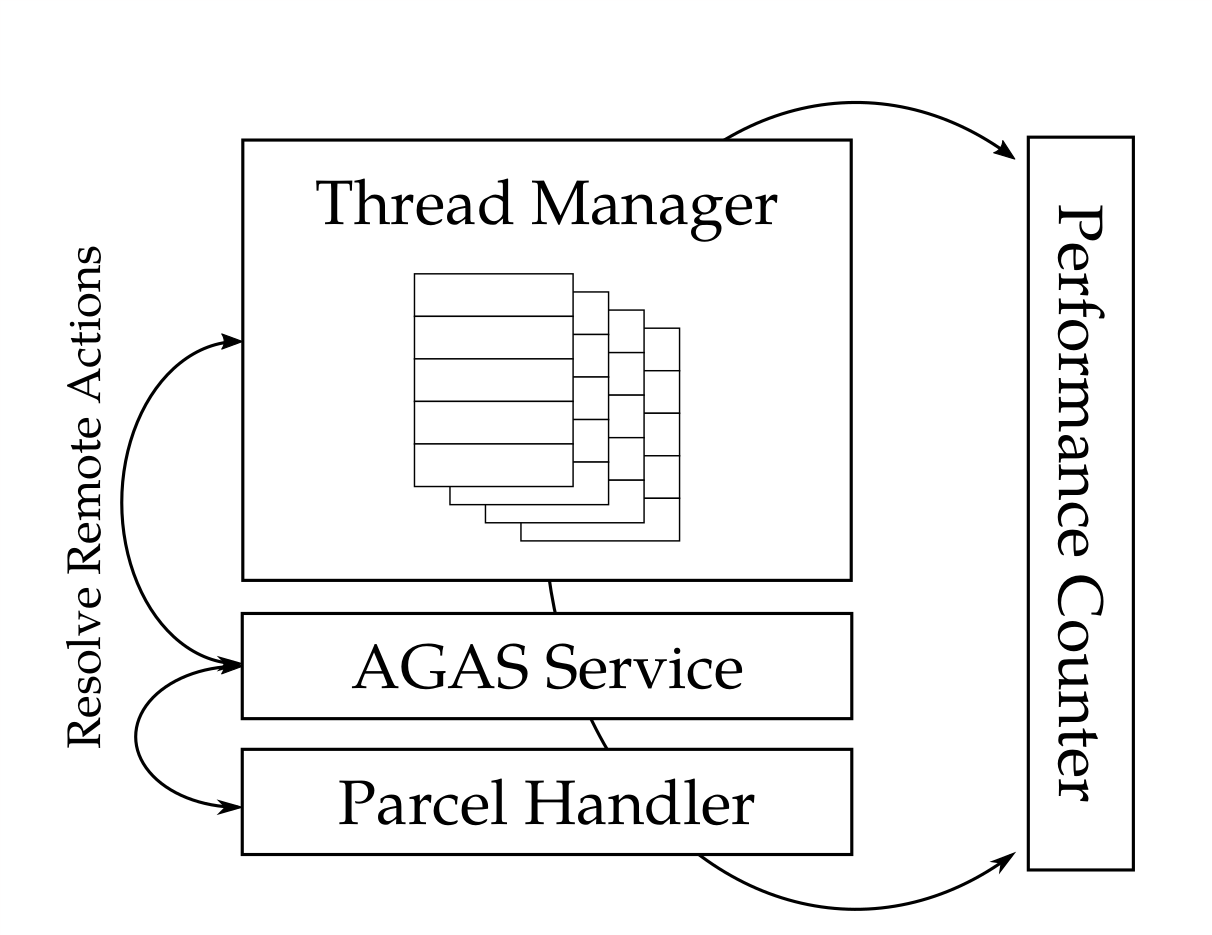
\includegraphics[width=50mm]{Figures/hpxArchitecture.png}
	 		\tiny T. Heller et al.: “Hpx – an open source c++ standard library for parallelism and concurrency” 2017.
		\normalsize
	\end{columns}
\end{frame}

% \subsection{HPX 101}
\begin{frame}
	\frametitle{Futures}
	\begin{center}
		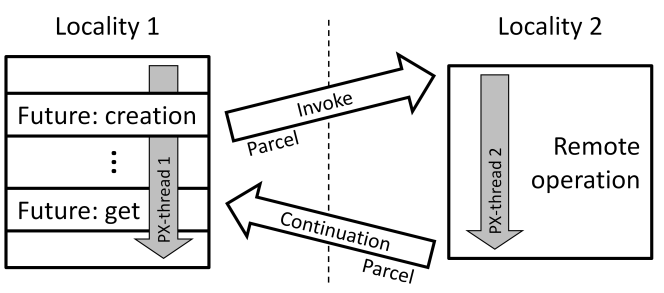
\includegraphics[width=100mm]{Figures/futureFlowDiagram.png}\\
		\tiny H. Kaiser et al.: “Parallex an advanced parallel
execution model for scaling-impaired applications” 2009.
		\normalsize
	\end{center}
\end{frame}

\begin{frame}
	\frametitle{Programming model}
	\begin{center}
		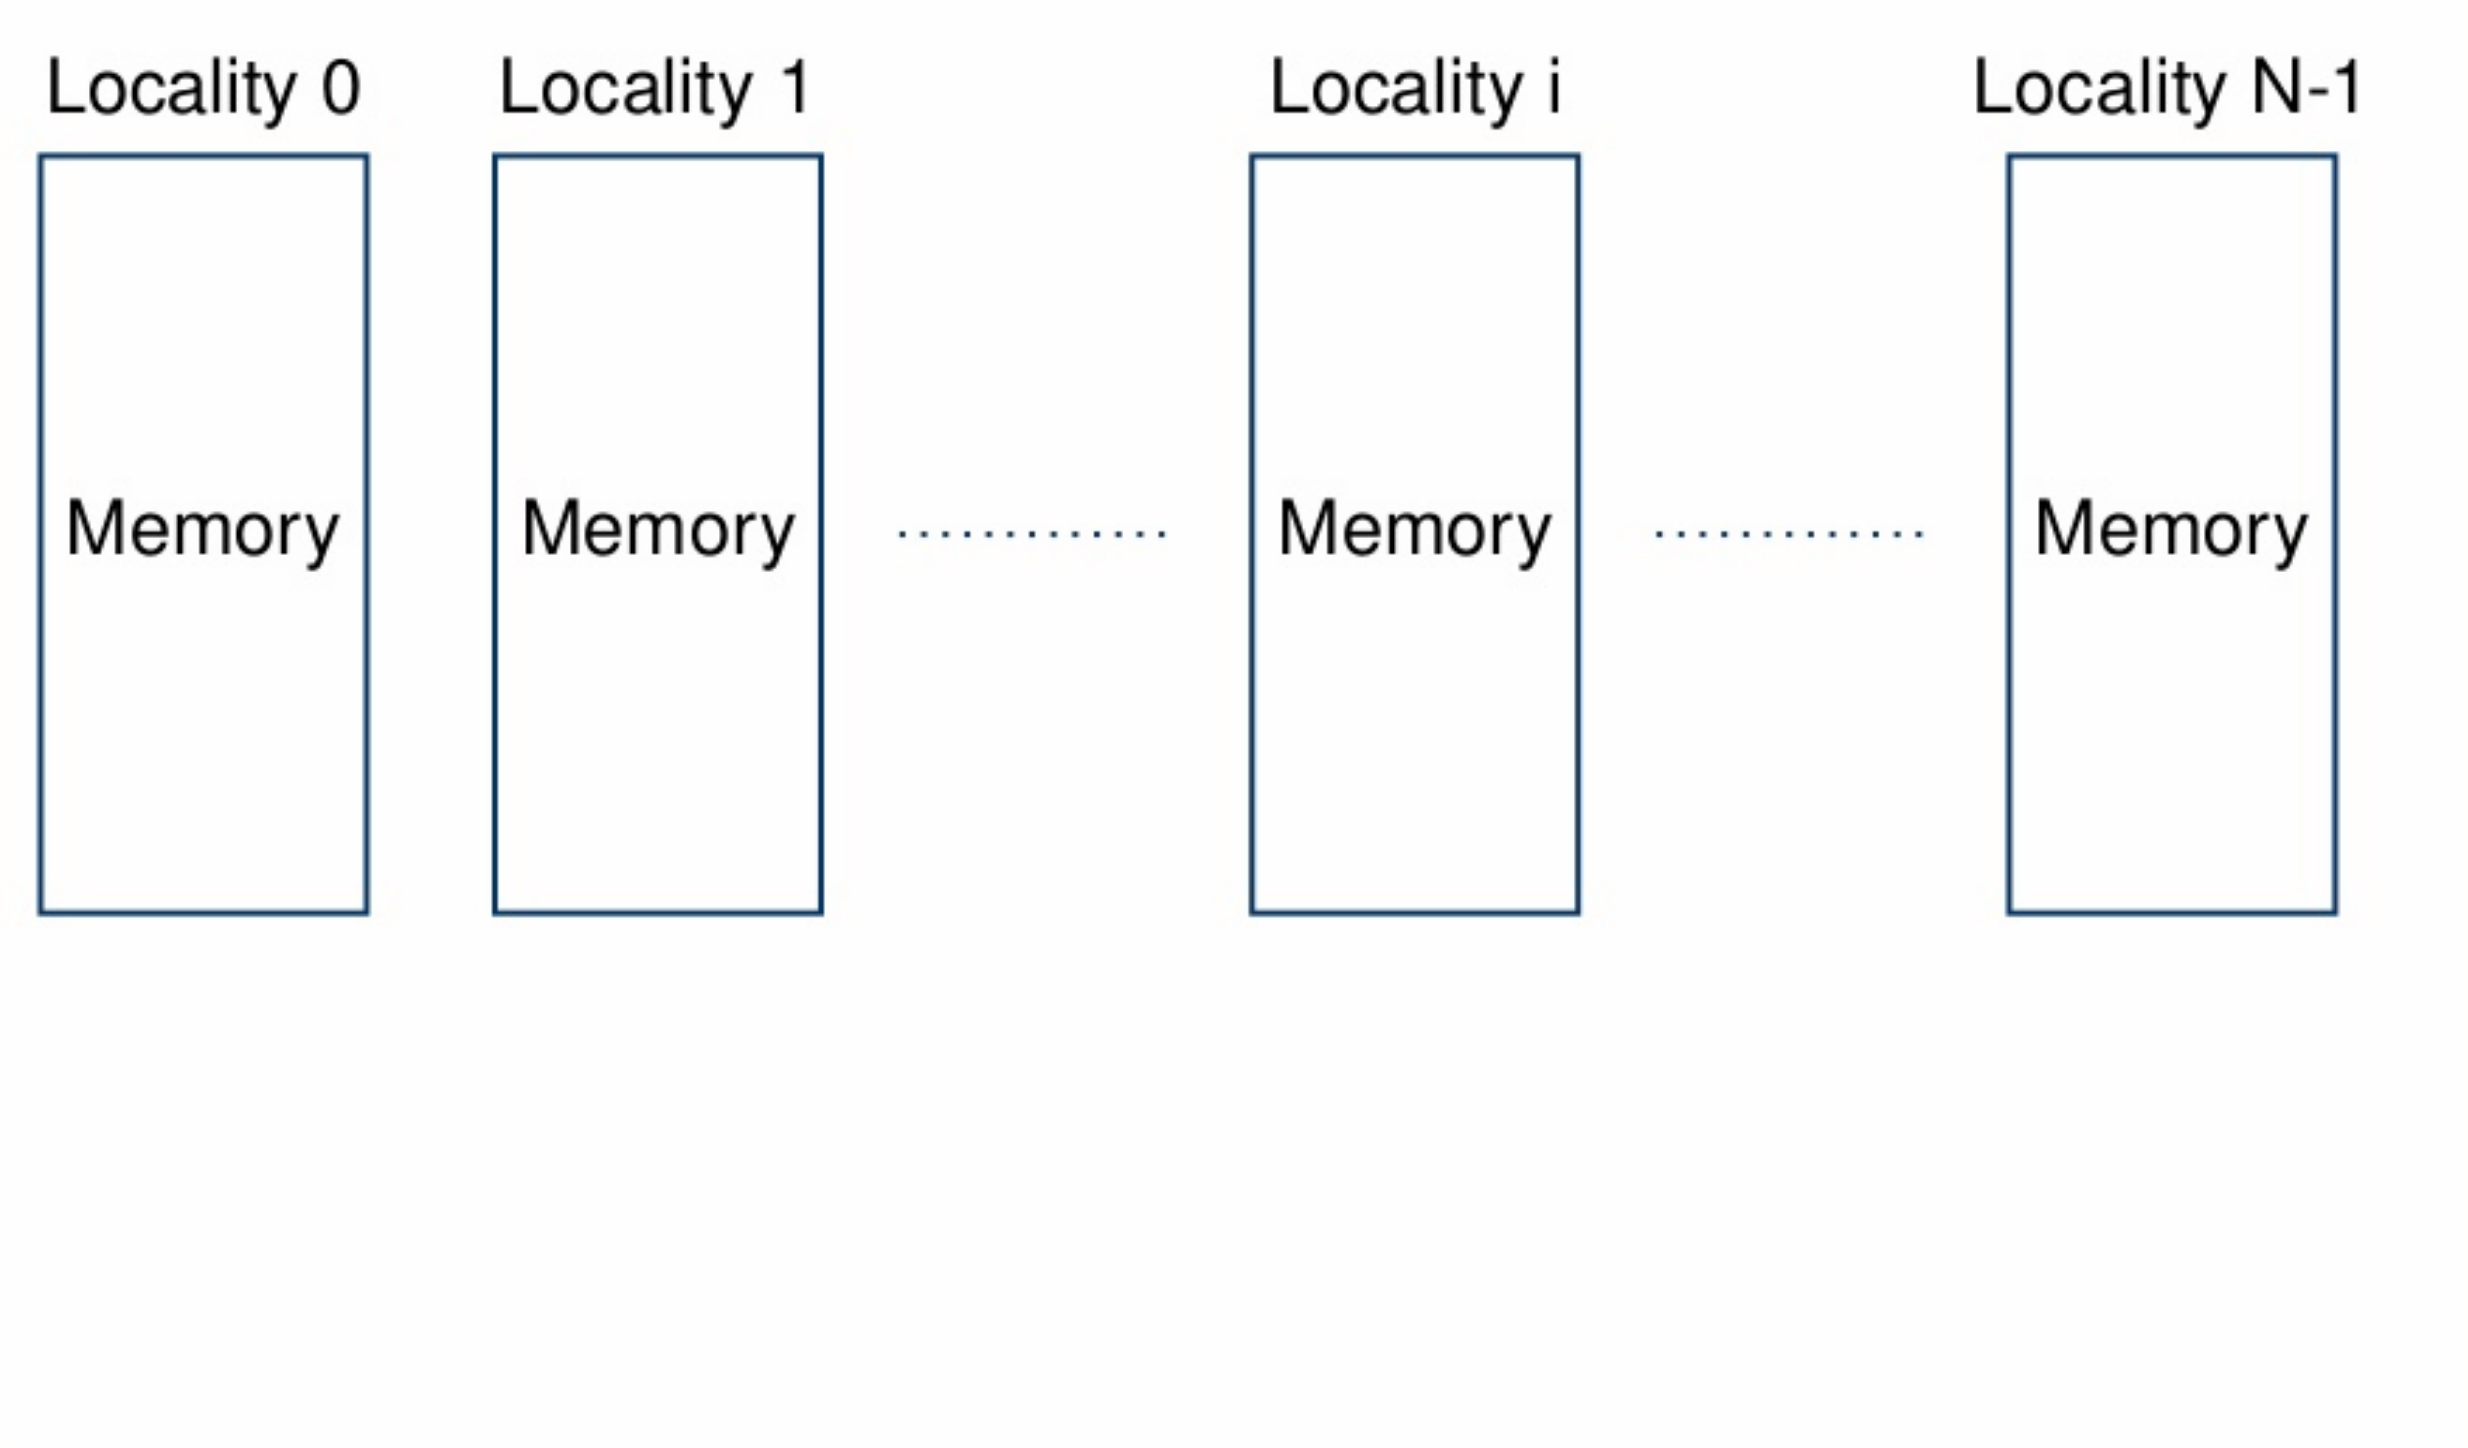
\includegraphics[width=100mm]{Figures/hpxProgrammingModel1.png}\\
		\vspace{3mm}
		\tiny T. Heller: “C++ on its way to exascale and beyond - The HPX Parallel Runtime System” 2016.
		\normalsize
	\end{center}
\end{frame}
\begin{frame}
	\frametitle{Programming model}
	\begin{center}
		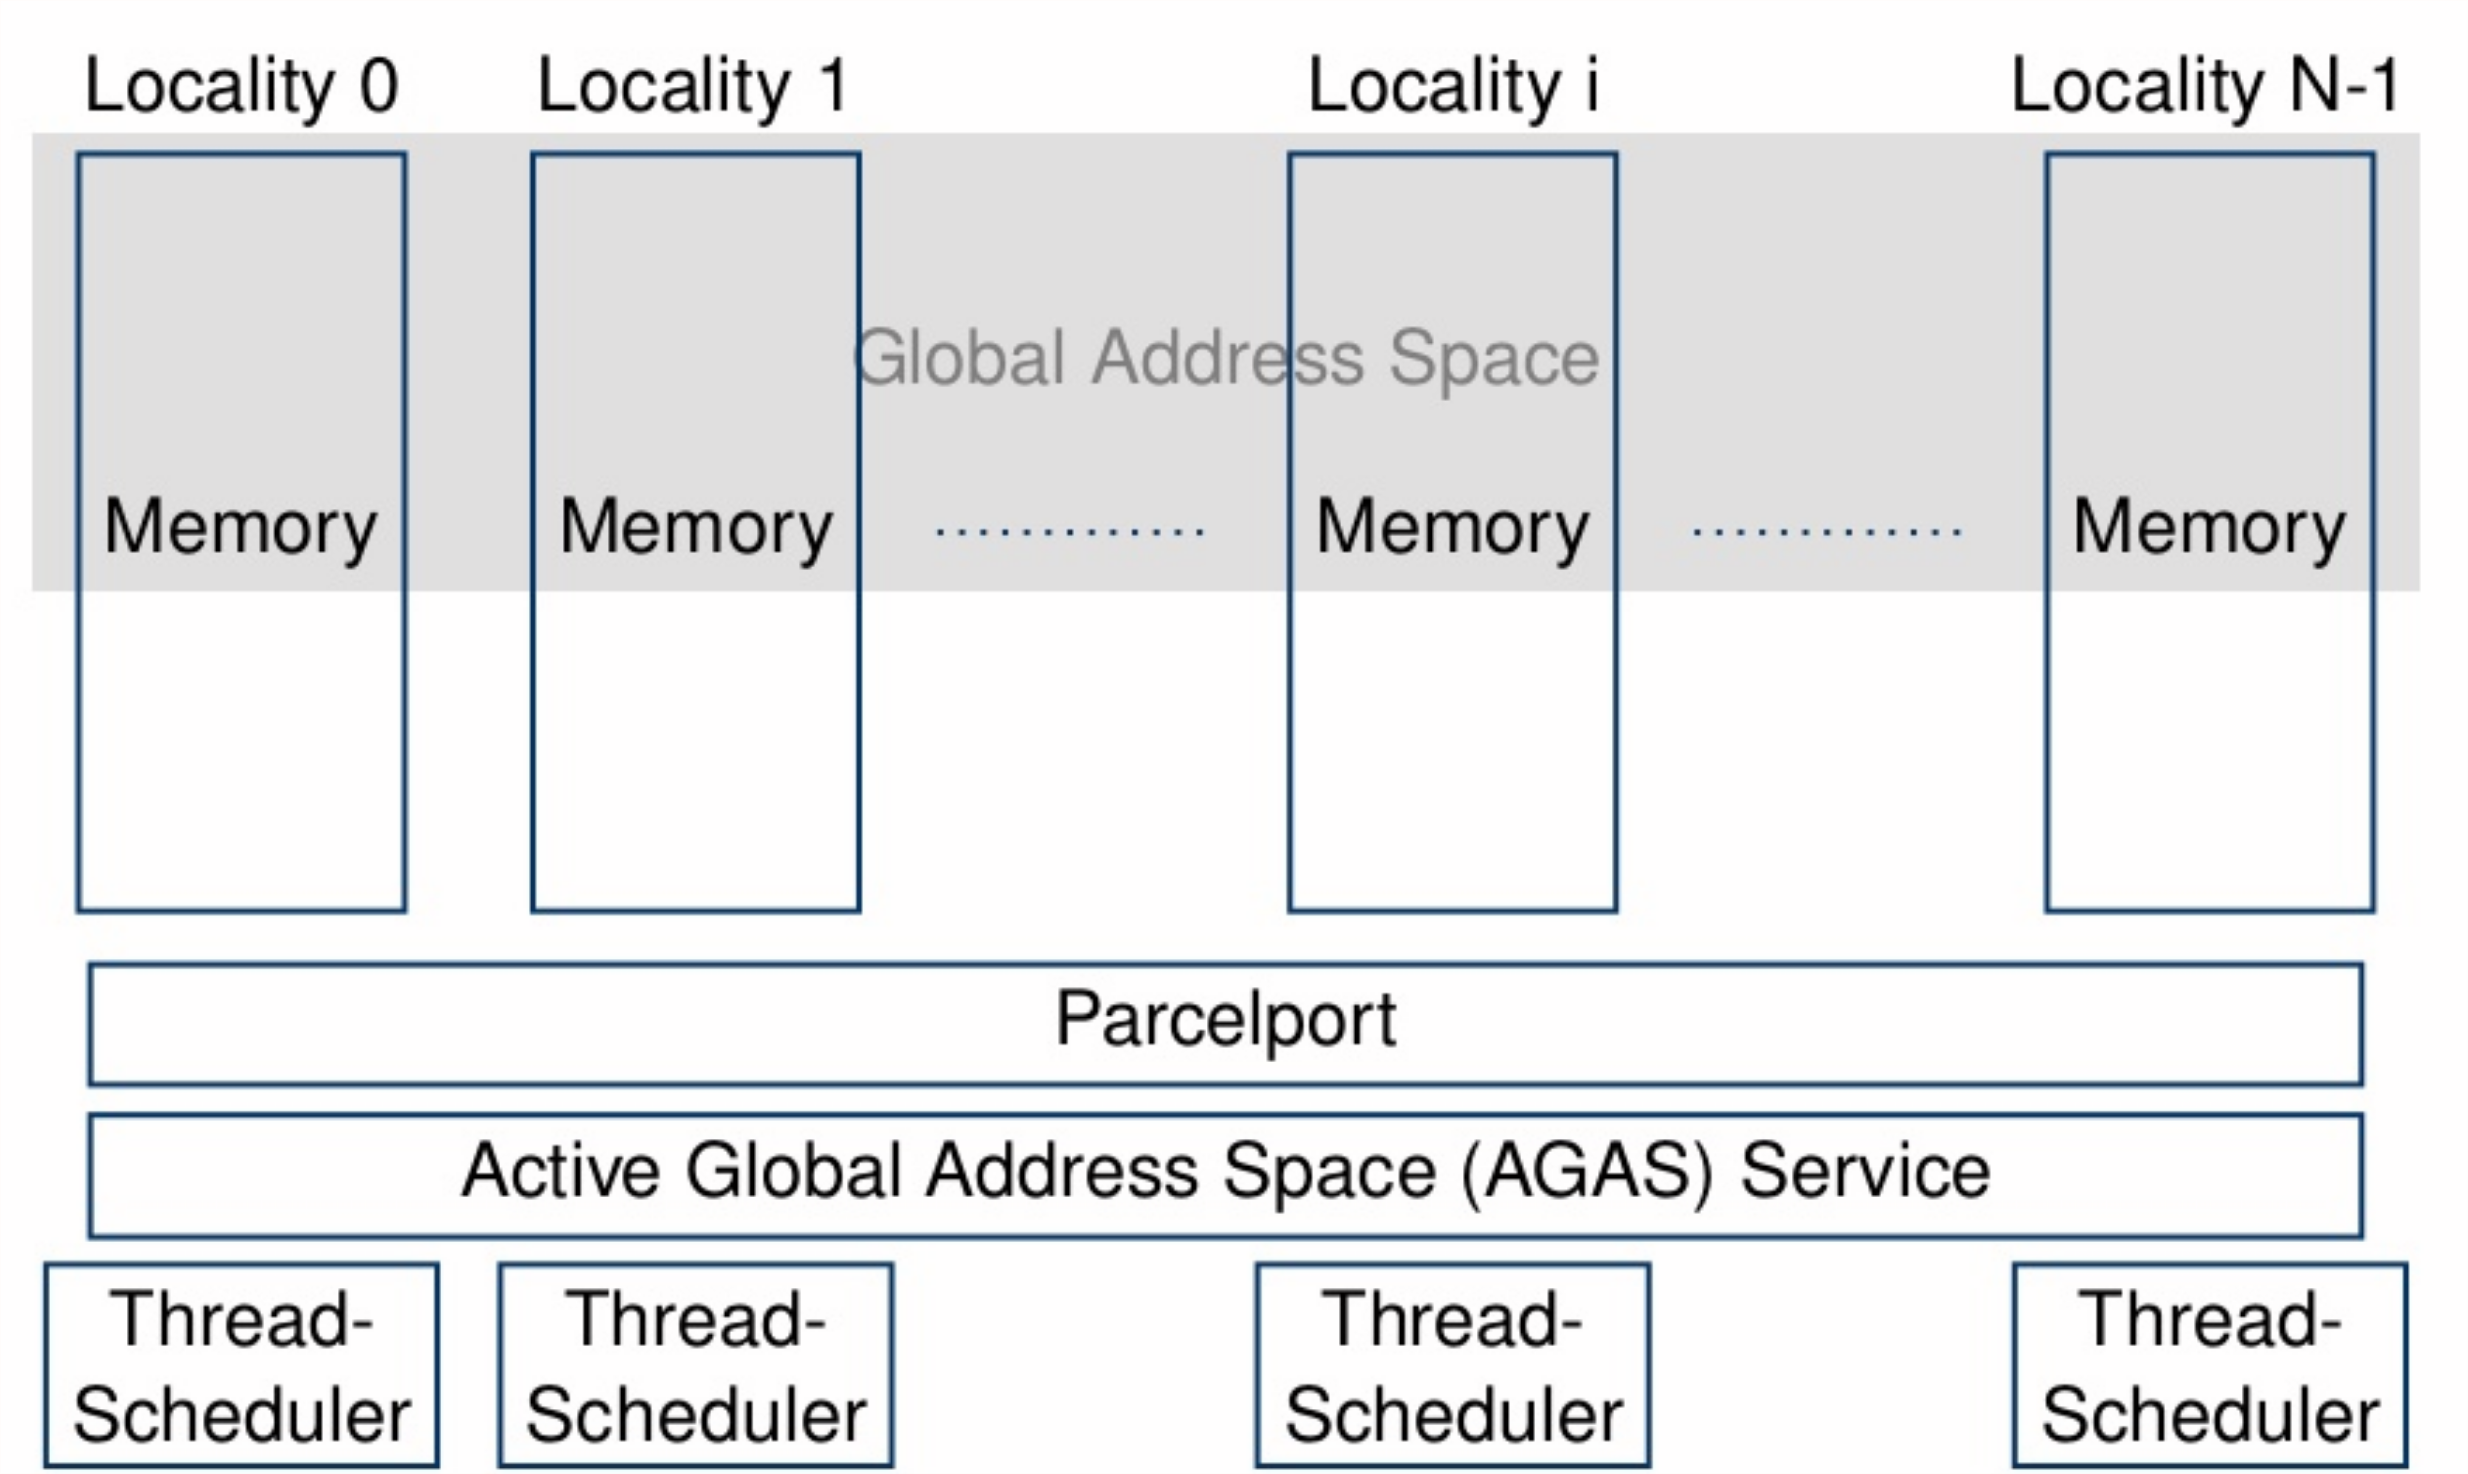
\includegraphics[width=100mm]{Figures/hpxProgrammingModel2.png}\\
		\vspace{3mm}
		\tiny T. Heller: “C++ on its way to exascale and beyond - The HPX Parallel Runtime System” 2016.
		\normalsize
	\end{center}
\end{frame}
\begin{frame}
	\frametitle{Programming model}
	\begin{center}
		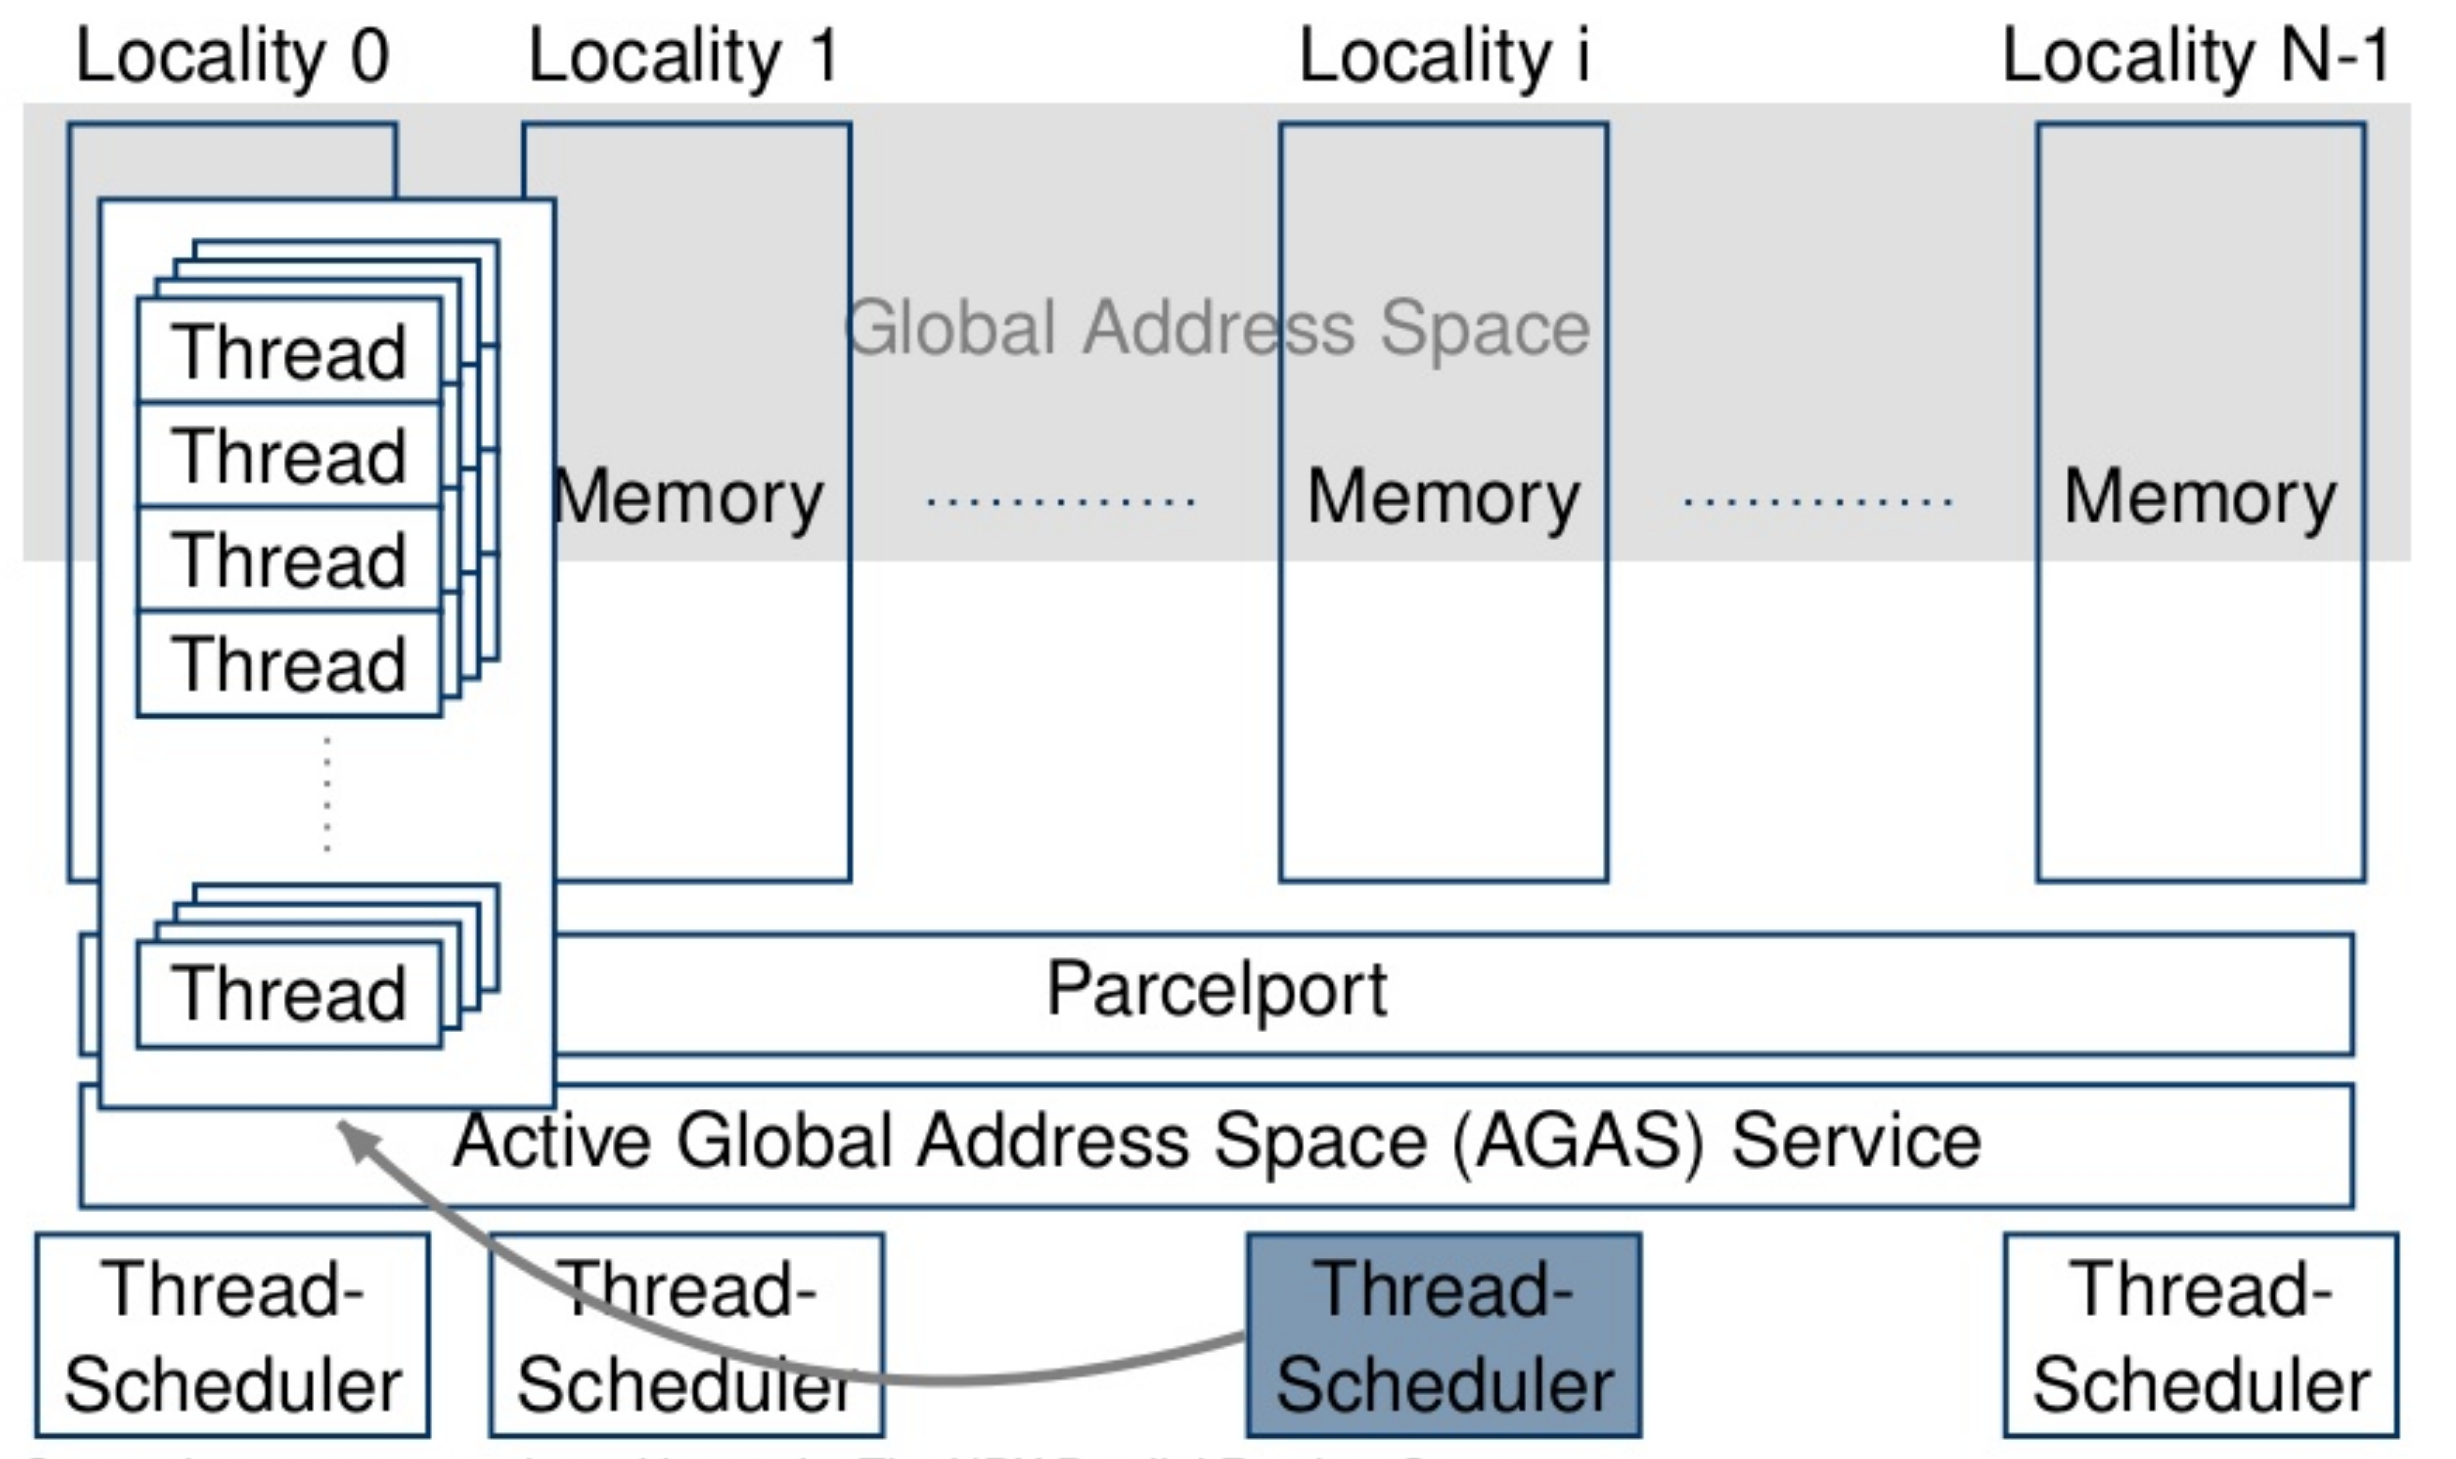
\includegraphics[width=100mm]{Figures/hpxProgrammingModel3.png}\\
		\vspace{3mm}
		\tiny T. Heller: “C++ on its way to exascale and beyond - The HPX Parallel Runtime System” 2016.
		\normalsize
	\end{center}
\end{frame}
\begin{frame}
	\frametitle{Programming model}
	\begin{center}
		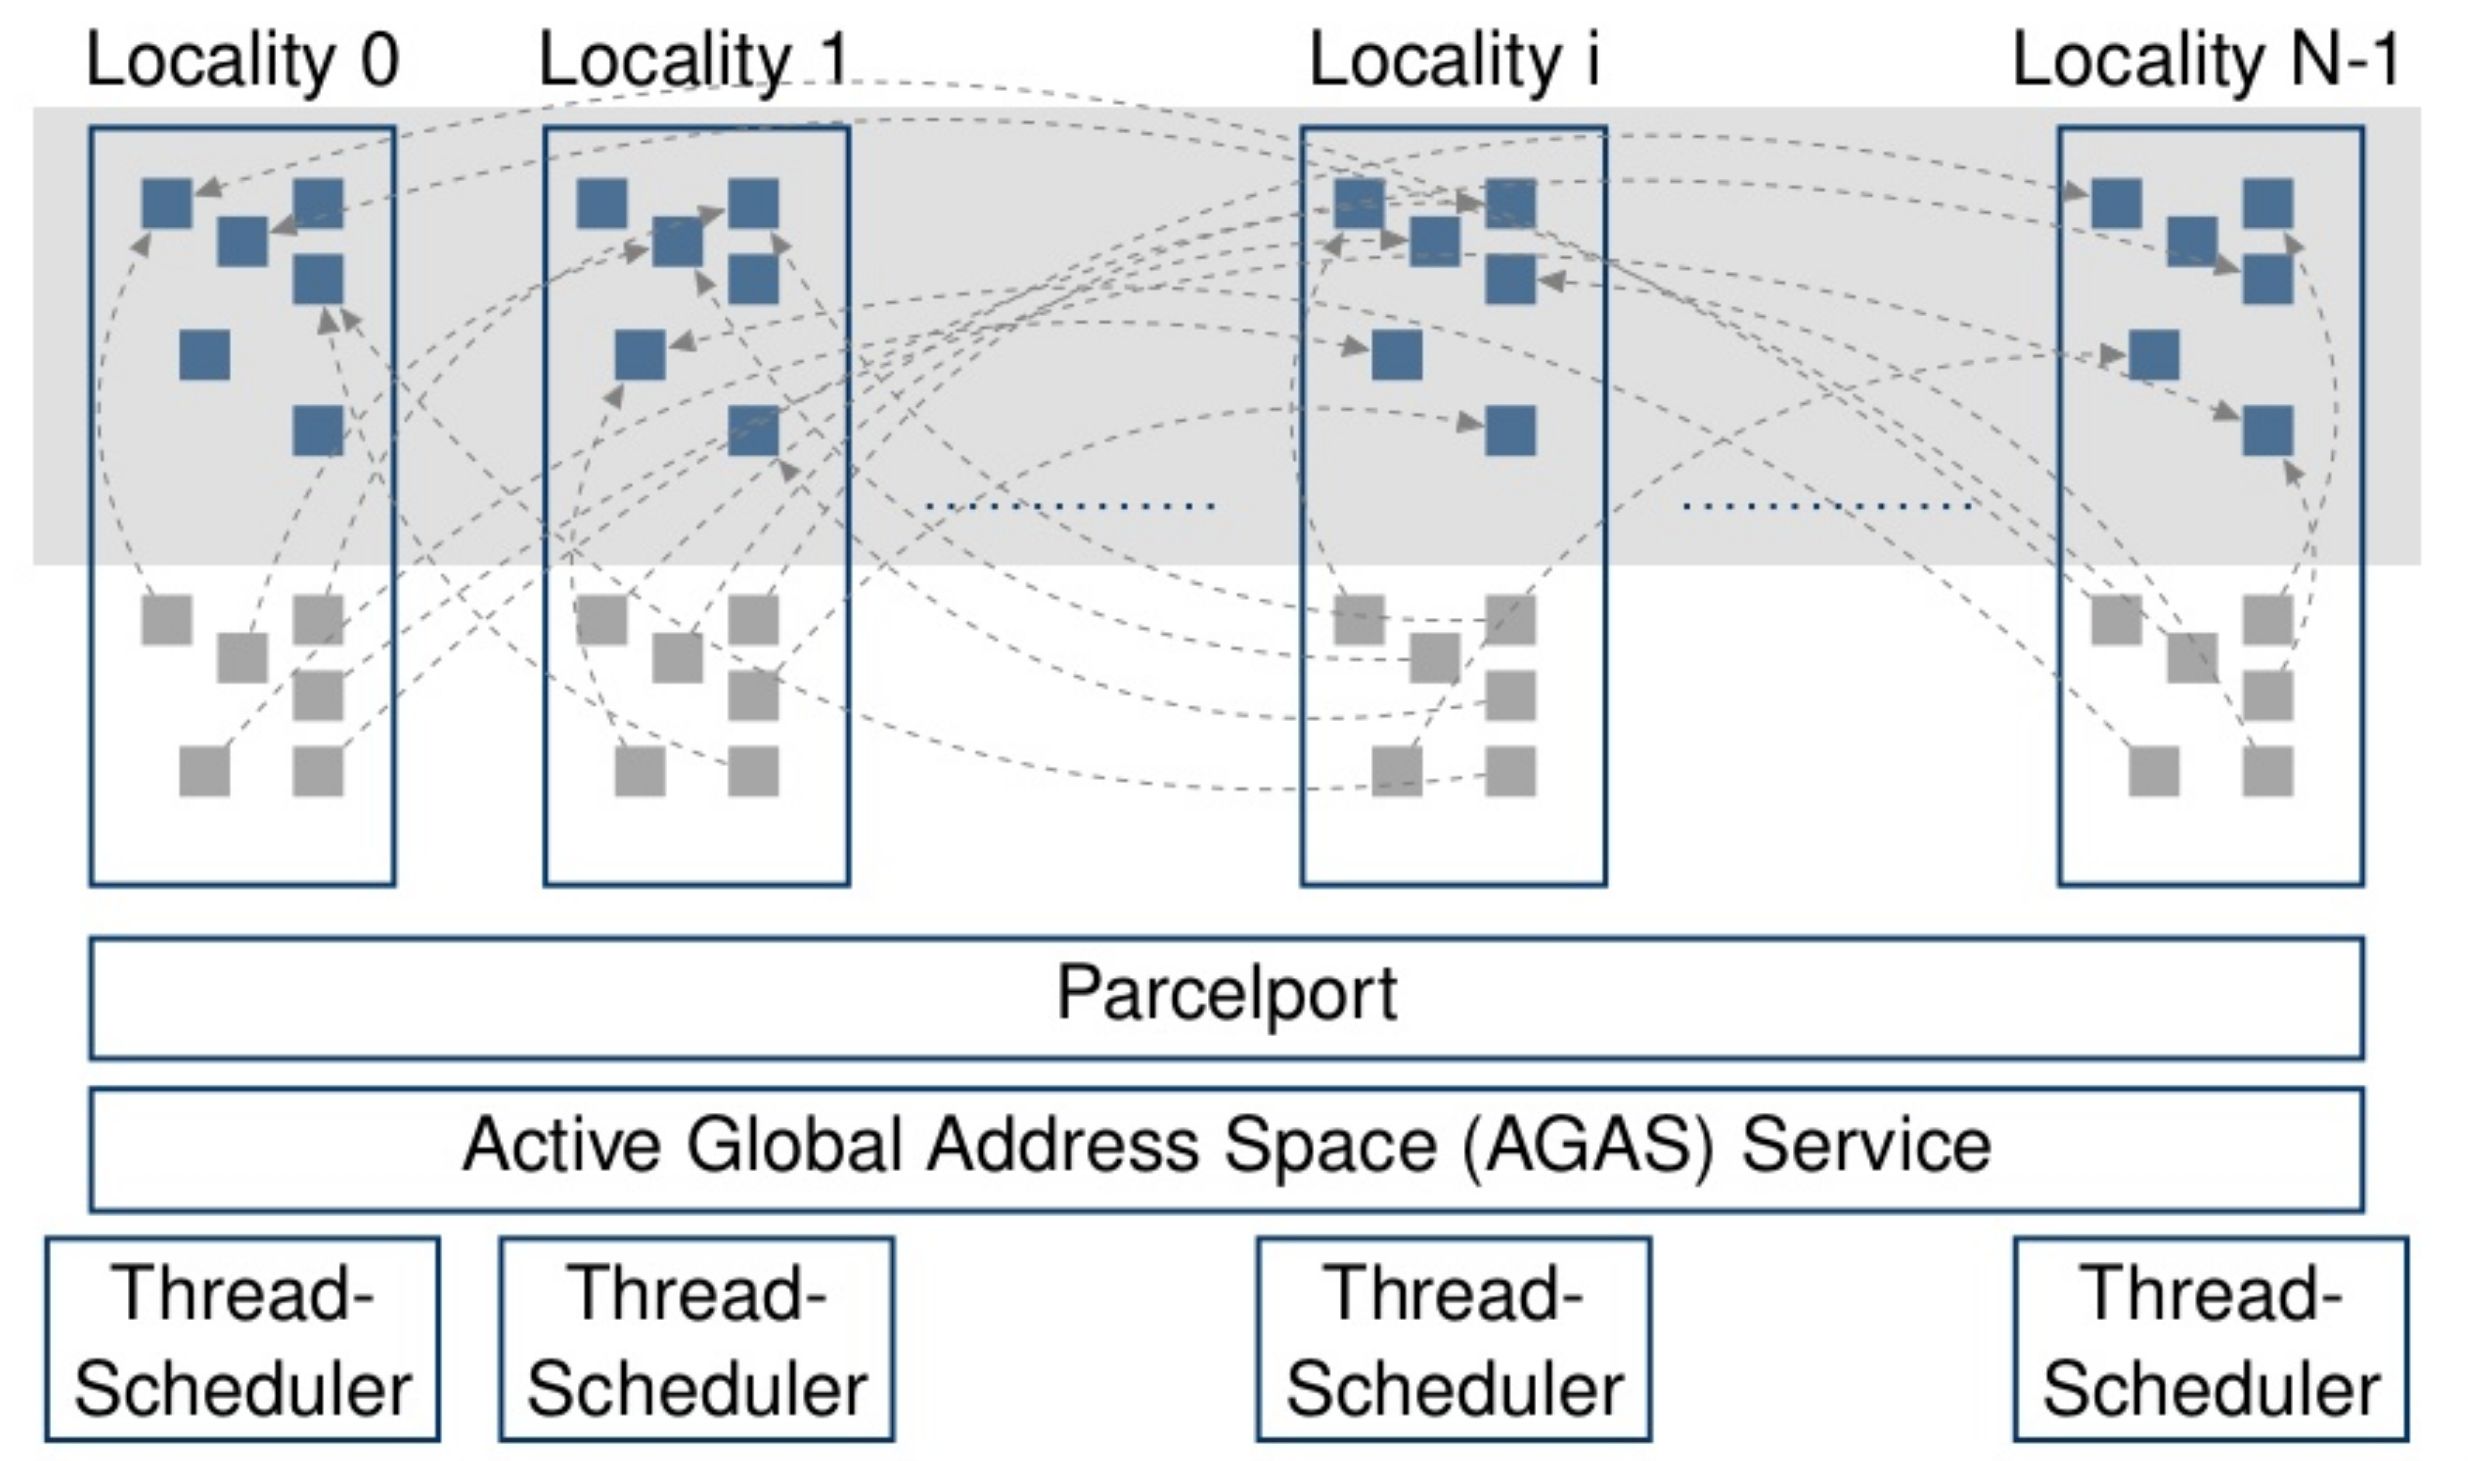
\includegraphics[width=100mm]{Figures/hpxProgrammingModel4.png}\\
		\vspace{3mm}
		\tiny T. Heller: “C++ on its way to exascale and beyond - The HPX Parallel Runtime System” 2016.
		\normalsize
	\end{center}
\end{frame}

\section{RA in HPX}
\begin{frame}
	\frametitle{HPX and Resource Awareness}
	\pause
	Capabilities
	\begin{enumerate}
		\item Task scheduling\\
			\small $\longrightarrow$ Work stealing + NUMA-awareness
		\normalsize
		\pause
		\item AGAS\\
			\small $\longrightarrow$ Dynamic relocation of objects
		\normalsize
		\pause
		\item Percolation\\
			\small $\longrightarrow$ Directly addressing HW accelerators
		\normalsize
		\pause
		\item Performance counters\\
			\small $\longrightarrow$ Allow easier integration of awareness into applications
		\normalsize
	\end{enumerate}
\end{frame}

\begin{frame}
	\frametitle{HPX and Resource Awareness (2)}
	Limitations
	\begin{itemize}
		\item (An)elasticity of HPX\\
			\small $\longrightarrow$ Worker threads and localities cannot be changed at runtime
		\normalsize
		\pause
		\item Energy unawareness\\
			\small $\longrightarrow$ E.g. no DVFS support
		\normalsize
		\pause
		\item Fault tolerance\\
			\small $\longrightarrow$ No built-in facility
		\normalsize
	\end{itemize}
\end{frame}

\section{Example}
\begin{frame}
	\frametitle{HPX coding example: the Mandelbrot set}
	% \begin{itemize}
	% 	\item Foo
	% \end{itemize}
	\begin{columns}
		\column{\dimexpr\linewidth-65mm-2mm}
		\pause
		\begin{equation*}
			\begin{cases}
				z_{c,0} &= 0 \\
				z_{c,n+1} &= z_{c,n}^2 + c
			\end{cases}
		\end{equation*}
		\pause
		\begin{align*}
			\mathcal{M} & = \\
			& \{c\in\mathbb{C} : \lim_{n\to\infty} |z_{c,n}| < +\infty \}
		\end{align*}
		\column{65mm}
		\begin{center}
			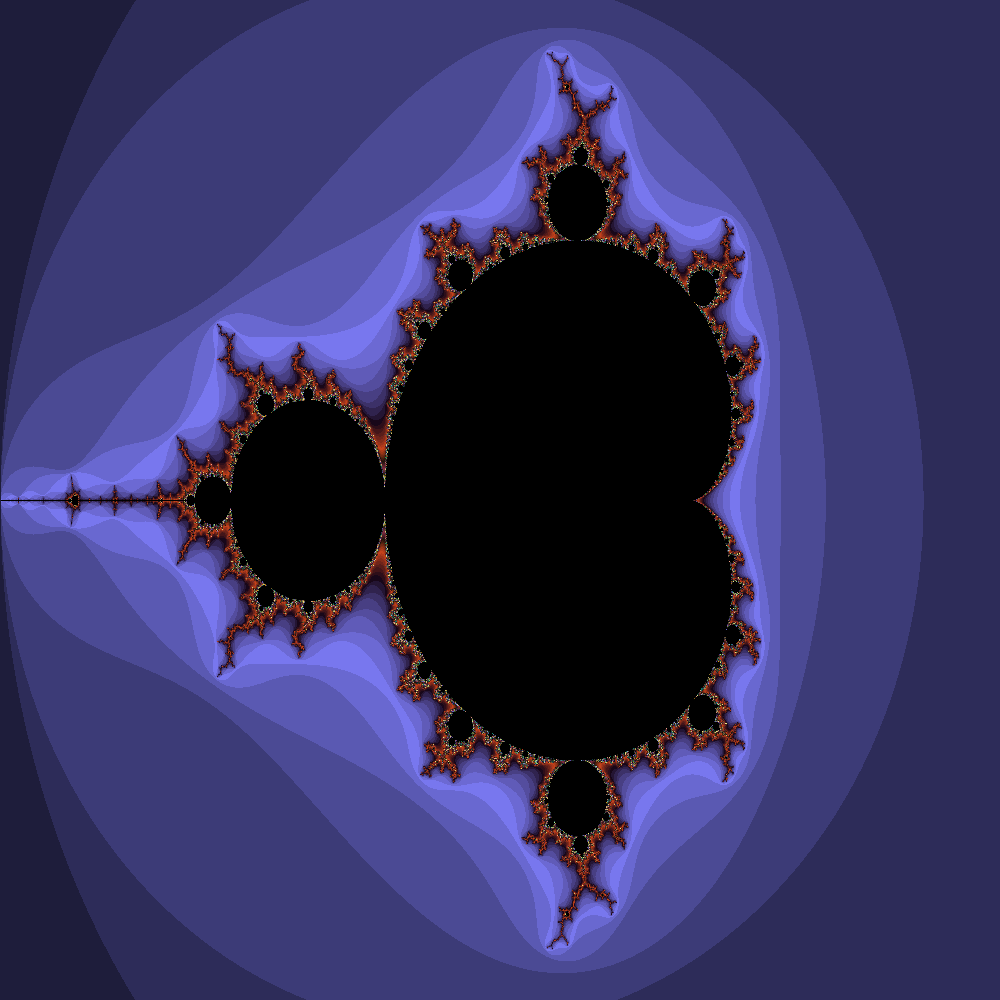
\includegraphics[width=65mm]{Figures/mandelbrot.png}
		\end{center}
	\end{columns}
\end{frame}

\begin{frame}[fragile]
	\frametitle{Mandelbrot: kernel}
\begin{lstlisting}[language=C]
void mandelbrot_kernel(int taskNo, staticData *sd) {
	// Computes one row of the image
	int i = taskNo;
	for (int j=0; j < sd->xRes; ++j) {
		int x = getX(j, sd);
		int y = getY(i, sd);
		complex double Z = 0 + 0*I;
		complex double C = x + y*I;
		
		int k = 0;
		do {	// Check the convergence of the sequence
			Z = Z * Z + C;
			k++;
		} while (cabs(Z) < 2 && k < max_iter);

		if (k == max_iter) {	// In case it did not diverge...
			memcpy(img[i][j], black, 3); //...we set a black pixel
		}
		else {	// If it diverged...
			//...we set the color according to k (#iterations)
			memcpy(img[i][j], getColor(k), 3);
		}
	}
}
\end{lstlisting}
\end{frame}

\begin{frame}[fragile]
	\frametitle{Mandelbrot: sequential code}
\begin{lstlisting}[language=C]
void mandelbrot_seq(...) {

	staticData *sd = assembleStaticData(...);

	// Iterate on rows, sequentially
	for (int i=0; i < yRes; ++i)
	{
		mandelbrot_kernel(i, sd);
	}
}
\end{lstlisting}
\end{frame}

\begin{frame}[fragile]
	\frametitle{Mandelbrot: futurized code}
	\begin{lstlisting}[language=C++]
void mandelbrot_hpx(...) {

	staticData *sd = assembleStaticData(...);

	std::vector<hpx::future<void>> futures;
	for (int i=0; i < yRes; ++i)
	{
		hpx::future<void> f = hpx::async(&mandelbrot_kernel, i, sd);
		futures.push_back(f);
	}

	hpx::wait_all(futures);
}
\end{lstlisting}
\end{frame}

\begin{frame}
	\frametitle{Mandelbrot step by step}
	\begin{center}
		% \animategraphics[loop,autoplay,scale=0.15]{10}{Figures/AnimatedMandelbrot/mandelbrot_}{00000}{000099}
		
\includegraphics[width=65mm]{Figures/mandelbrot_partial.png}
	\end{center}
\end{frame}

\section{Summary}
\begin{frame}
	\frametitle{Summary}
	\begin{itemize}
		\item Future exascale computing requires smart code.
		\item Resource awareness can be a way to achieve better performance.
		\item HPX has the potential to become a major runtime system for HPC, thanks to both its performance and programmability.
	\end{itemize}
	\pause
	\vspace{5mm}
	\begin{center}
		\LARGE Thanks! \normalsize
	\end{center}
\end{frame}

%%%%%%%

% \begin{frame}
% 	\frametitle{Title}
% 	\begin{itemize}
% 		\item Foo
% 	\end{itemize}
% \end{frame}

\end{document}
